%Q 23|ACJC 2023 Prelim P2 Q11
\defQ{23}{}{%
Energy bars are a convenient source of nutrition for athletes. A typical energy bar weighs between 30-50 g and is likely to supply about 200-300 calories. An American company sells energy bars and a nutritionist working in the company claims that the mean number of calories in a product, Perfect Protein bars, is 350 calories.\par
A random sample of 30 bars is collected and the number of calories, $x$ cal, in the 30 bars is summarised as follows.
\[\textstyle\sum x=10446,\qquad \sum x^2=3638000.\]
\begin{qparts}
\pt{(i)} Test at the 3\% level of significance whether the mean number of calories in Perfect Protein bars is less than 350 calories, defining any symbols that you use. \mk{7}
\pt{(ii)} Explain why the test would be inadmissible if the nutritionist had taken a random sample of 15 energy bars and hence state an assumption needed for him to carry out the test. \mk{1}
\pt{(iii)} If the test was for whether the mean number of calories in Perfect Protein bars is 350 calories, find the smallest level of significance for which the nutritionist's claim will be rejected. \mk{2}
\end{qparts}
The company launched a new product called Dynamic Protein bars which are advertised to be higher in calories than Perfect Protein bars. A random sample of 45 Dynamic Protein bars is collected to test this and the mean number of calories of the sample is found to be 352.2.
\begin{qparts}
\pt{(iv)} The result of this investigation shows that there is no reason to believe that the mean number of calories in the new product is more than 350 calories at the 4\% level of significance. Find the range of possible values of the variance used in calculating the test statistic. \mk{3}
\end{qparts}
\src{ACJC 2023 Prelim P2 Q11}}
\defS{23}{%
\pt{(i)} $\bar{x}=\dfrac{\sum x}{n}=\dfrac{10446}{30}=348.2$ (exact)\par
$s^2=\dfrac{1}{n-1}\left(\sum x^2-\dfrac{\left(\sum x\right)^2}{n}\right)=\dfrac{1}{29}\left(3638000-\dfrac{(10446)^2}{30}\right)=24.23448$\par
Let $\mu$ be the population mean number of calories in Perfect Protein bars.\par\medskip
Null hypothesis \qquad $H_0:\ \mu=350$\par
Alternative hypothesis \quad $H_1:\ \mu<350$\par
Perform 1-tail test at 3 \% significance level.\par\medskip
Under $\mathrm{H}_0$, $\bar{X}\sim\mathrm{N}\left(350\,,\dfrac{24.23448}{30}\right)$ by Central Limit Theorem since $n=30$ is large enough.\par\medskip
From GC, $z=\dfrac{\bar{x}-\mu_0}{\sqrt{\dfrac{s^2}{n}}}=\dfrac{348.2-350}{\sqrt{\dfrac{24.23448}{30}}}=-2.0027$\par
\qquad\qquad $p$-value $=P\left(Z<-2.0027\right)=0.0226$
\htz{-2.0027}{none}{$-2.0027$}{}{0.0226}{}
$p$-value $<0.03$ $\therefore$Reject $\mathrm{H}_0$\par
There is sufficient evidence at 3\% level of significance to conclude that the mean number of calories in Perfect Protein bars is less than 350 cal.
\pt{(ii)} The test would be inadmissible if the nutritionist had taken a random sample of 15 energy bars as the distribution of the population is unknown (and Central Limit Theorem cannot be applied). The nutritionist will need to assume that the number of calories in Perfect Protein bars follow a normal distribution.
\pt{(iii)} Null hypothesis \qquad $\mathrm{H}_0:\ \mu=350$\par
Alternative hypothesis \quad $\mathrm{H}_1:\ \mu\neq350$\par
Perform 2-tail test at $\alpha$ \% significance level.\par\medskip
$p$-value $=2\times P\left(Z<-2.0027\right)=0.0452$\par
To reject $\mathrm{H}_0$, $p$-value $=0.045209<\alpha\%$\par
$\therefore$ smallest significance level is 4.52\%.
\pt{(iv)} Let $\mu$ be the population mean number of calories in Dynamic Protein bars.\par\medskip
Null hypothesis \qquad $H_0:\ \mu=350$\par
Alternative hypothesis \quad $H_1:\ \mu>350$\par
At 4\% level of significance, we do not reject $H_0$.\par\medskip
For $p$-value $>0.04$ or $z<1.750686$, we do not reject $H_0$.\par
$z=\dfrac{\bar{x}-\mu_0}{\sqrt{\dfrac{\sigma^2}{n}}}=\dfrac{352.2-350}{\sqrt{\dfrac{\sigma^2}{45}}}<1.750686$
\htz{none}{1.75068}{}{1.75068}{}{0.04}
$1.750686\sqrt{\dfrac{\sigma^2}{45}}>2.2$\par
$\sigma^2>45\left(\dfrac{2.2}{1.750686}\right)^2$\par
$\sigma^2>71.0626$\par
$\therefore\sigma^2>71.1$ (3 sf.)
}
%Q 24|VJC 2025 Prelim P2 Q12
\defQ{24}{}{%
A hospital introduces a new medication regimen to help patients recover from a viral infection more quickly. Previously, the average recovery time was 7.2 days.\par
After adopting the new regimen, a random sample of 40 patients is observed, and their recovery times, $x$, in days, are recorded. The results are summarised below.
\[\textstyle\sum(x-7.2)=-42\quad\text{and}\quad\sum(x-7.2)^2=648\]
\begin{qparts}
\pt{(a)} Explain whether the hospital should carry out a one-tailed test or a two-tailed test. \mk{1}
\pt{(b)} Calculate unbiased estimates of the population mean and variance of the recovery times under the new regimen. \mk{2}
\pt{(c)} Carry out an appropriate test at the 5\% significance level. You should state clearly the hypotheses for your test and define any parameters that you use. \mk{4}
\pt{(d)} Explain, in the context of the question, the meaning of `at the 5\% significance level'. \mk{1}
\pt{(e)} Explain whether it would have been sufficient for the hospital to take a random sample of 10 patients and record their recovery times under the new regimen in order to carry out the hypothesis test. \mk{1}
\end{qparts}
It was discovered that an intern at the hospital had made an error in recording the recovery times. A random sample of another 30 patients was taken and their recovery times under the new regimen was taken and recorded by a senior researcher. The sample standard deviation was found to be 1.7 days and the sample mean time was denoted by $k$.
\begin{qparts}
\pt{(f)} A test at the 1\% significance level concludes that the average recovery time did not improve from 7.2 days. Find the set of values of $k$. \mk{3}
\end{qparts}
\src{VJC 2025 Prelim P2 Q12}}
\defS{24}{%
\pt{(a)} The researchers should carry out a one-tailed test as they want to test whether the new regimen has \textbf{reduced mean recovery time.}
\pt{(b)} Let $y=x-7.2$\par
Unbiased estimate of population mean, $\bar{x}=\bar{y}+7.2=\dfrac{-42}{40}+7.2=6.15$\par
Unbiased estimate of population variance,\par
$s_x^2=s_y^2=\dfrac{1}{39}\left(648-\dfrac{(-42)^2}{40}\right)=\dfrac{603.9}{39}=15.4846\approx15.5$
\pt{(c)} Let $X$ days be the recovery time of a patient and $\mu$ days be the population mean of $X$.\par
$\mathrm{H}_0:\mu=7.2$\par
$\mathrm{H}_1:\mu<7.2$\par
Level of Significance: 5\%\par\medskip
Test Statistic:\par
Since $n=40$ is large, $\bar{X}\sim\mathrm{N}\left(7.2,\dfrac{15.4846}{40}\right)$ approximately by CLT.\par
When $\mathrm{H}_0$ is true, $Z=\dfrac{\bar{X}-7.2}{S/\sqrt{n}}\sim\mathrm{N}(0,1)$ approximately.\par\medskip
Computation: $\bar{x}=6.15$, $s_x^2\approx15.4846$, $p$-value $=0.045744$ (or $z=-1.6876$)
\htz{-1.6876}{none}{$-1.6876$}{}{0.0457}{}
Conclusion: Since $p$-value $=0.0457<0.05$, $\mathrm{H}_0$ is rejected at 5\% level of significance. Hence there is sufficient evidence to conclude that the mean recovery time has reduced under the new regimen.
\pt{(d)} A 5\% significance level means that there is a probability of 0.05 that the test concludes that the mean recovery time has reduced when it is actually 7.2 days.
\pt{(e)} No. Since the distribution of recovery time under the new regimen ($X$) is unknown, the sample size would have to be sufficiently large for Central Limit Theorem to be applied so that the \textbf{sample mean recovery time} is approximately normally distributed. A sample of 10 is not large enough.
\pt{(f)} $\mathrm{H}_0:\mu=7.2$\par
$\mathrm{H}_1:\mu<7.2$\par
Level of Significance: 1\%\par
Test Statistic:\par
Since $n=30$ is large, $\bar{X}\sim\mathrm{N}\left(7.2,\dfrac{2.9897}{30}\right)$ approximately by CLT.\par
When $\mathrm{H}_0$ is true, $Z=\dfrac{\bar{X}-7.2}{S/\sqrt{n}}\sim\mathrm{N}(0,1)$ approximately.\par\medskip
Computation:\par
$s^2=\dfrac{n}{n-1}(\text{sample variance})=\dfrac{30}{29}(1.7)^2=2.9897$\par\medskip
Rejection Region: $z\leq-2.3263$
\htz{-2.3263}{none}{$-2.3263$}{}{0.01}{}
Since $\mathrm{H}_0$ is not rejected,\par
$\dfrac{k-7.2}{\sqrt{2.9897}\big/\sqrt{30}}>-2.3263$\par
$k>6.4656$\par\medskip
$\therefore\{k\in\mathbb{R}:k>6.47\}$
}
%Q 25|JPJC 2024 Prelim P2 Q10
\defQ{25}{}{%
In a drinks factory, a machine is programmed to dispense 500 ml of green tea into empty bottles.
\begin{qparts}
\pt{(a)} After a routine check of the machine, the production manager suspects that the machine is dispensing more green tea than expected. A random sample of 50 bottles is taken for a hypothesis test at $\alpha$\% level of significance and the data is as follows:\par\smallskip
{\centering\begin{tabular}{|l|c|c|c|c|c|c|c|}\hline
\begin{tabular}{@{}l@{}}Volume of green tea\\(correct to nearest ml)\end{tabular} & 498 & 499 & 500 & 501 & 502 & 503 & 504\\\hline
Number of bottles & 5 & 11 & 10 & 11 & 10 & 1 & 2\\\hline\end{tabular}\par}\smallskip
Taking $\alpha=2$, test the production manager's suspicion and state the meaning of the $p$-value in the context of the question. \mk{5}
\pt{(i)} Determine the set of values of $\alpha$ for which the production manager's suspicion is valid. \mk{1}
\pt{(ii)} Explain why the production manager is able to carry out the hypothesis test without knowing anything about the distribution of the volume of green tea dispensed by the machine. \mk{1}
\pt{(b)} The machine is being recalibrated to dispense 500 ml of green tea. Another random sample of 50 bottles of green tea is taken and the mean and standard deviation of this sample are 502 ml and $k$ ml respectively. A hypothesis test, at the 5\% significance level, concluded that the recalibration is done accurately. Find the set of values that $k$ can take. \mk{5}
\end{qparts}
\src{JPJC 2024 Prelim P2 Q10}}
\defS{25}{%
\pt{(a)}{\centering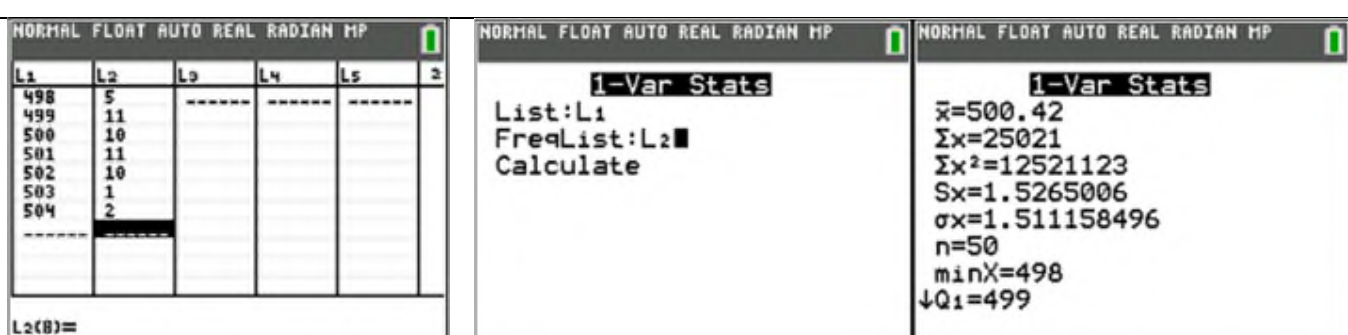
\includegraphics[width=0.98\linewidth]{gc_jpjc_1.png}\par}
Using GC,\par
$\bar{x}=500.42$ (exact)\par
$s=1.5265$ (to 5 s.f.)\par
{\centering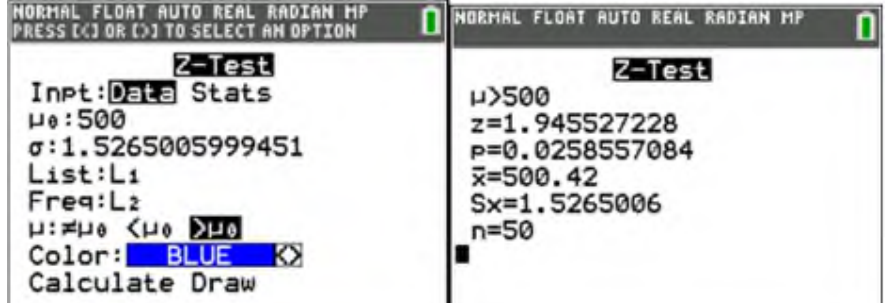
\includegraphics[width=0.66\linewidth]{gc_jpjc_2.png}\par}
Let $X$ = vol. of green tea dispensed in a bottle and\par
\quad $\mu$ = population mean green tea dispensed in a bottle\par
$\mathrm{H}_0:\mu=500$\par
$\mathrm{H}_1:\mu>500$\par
Under $\mathrm{H}_0$ ,since $n$ = 50 is large, by Central Limit Theorem,\par
\qquad $\bar{X}\sim\mathrm{N}\left(500\ ,\ \dfrac{1.5265^2}{50}\right)$ approximately\par
Test statistic: $z=\dfrac{\bar{x}-500}{\left(\dfrac{1.5265}{\sqrt{50}}\right)}$\par
\qquad\qquad\quad $=\dfrac{500.42-500}{\left(\dfrac{1.5265}{\sqrt{50}}\right)}=1.9455\approx1.95$ (to 3 s.f)\par
From GC, $p$-value = $0.025856\approx0.0259$ (to 3 s.f)
\htz{none}{1.9455}{}{1.95}{}{0.0259}
Since $p$-value = 0.0259 $>$ 0.02, we do not reject $\mathrm{H}_0$ at 2\% level of significance and conclude that there is insufficient evidence that the production manager's suspicion is valid.\par\medskip
The $p$-value is 0.0259 and it means there is a probability of 0.0259 of observing a test statistic, $z\geq1.95$, given that the population mean green tea dispensed in a bottle is 500ml.
\pt{(i)} For the production manager's suspicion ($\mu>500$) to be valid, $\mathrm{H}_0$ is rejected. Hence,\par
$p$-value = $0.025856<\dfrac{\alpha}{100}$\par
\qquad $\therefore2.59<\alpha<100$ (3 s.f)
\pt{(ii)} Since the sample size = 50 is large enough, Central Limit Theorem can be applied for sample means to follow a normal distribution approximately.
\pt{(b)} $s^2=\dfrac{n}{n-1}\sigma_x^{\,2}=\dfrac{50}{49}k^2$\par
$\mathrm{H}_0:\mu=500$\par
$\mathrm{H}_1:\mu\neq500$\par
Under $\mathrm{H}_0$ ,since $n$ = 50 is large, by Central Limit Theorem,\par
\qquad $\bar{X}\sim\mathrm{N}\left(500\ ,\ \dfrac{\left(\frac{50k^2}{49}\right)}{50}\right)=\mathrm{N}\left(500\ ,\ \dfrac{k^2}{49}\right)$ approximately\par
Test statistic: $z=\dfrac{\bar{x}-500}{\sqrt{\dfrac{k^2}{49}}}=\dfrac{502-500}{\dfrac{k}{7}}=\dfrac{14}{k}$\par
For $\alpha$ = 0.05,
\htz{-1.95996}{1.95996}{$-1.95996$}{$1.95996$}{}{}
If recalibration is done accurately ($\mu=500$), $\mathrm{H}_0$ is not rejected. Hence,\par
$-1.95996<z<1.95996$\par
\qquad $-1.95996<\dfrac{14}{k}<1.95996$\par
$\dfrac{k}{14}<-0.51021$ (rejected) \ or \ $\dfrac{k}{14}>0.51021$\par
\qquad\qquad\qquad\qquad\qquad\qquad $k>7.1430$\par
\qquad\qquad\qquad\qquad\qquad $\therefore k>7.14$ \ (to 3 s.f)\par\smallskip
{\color{black!55}\footnotesize[Note: the official solution labels the parts 10(i), (ii), (iii), (b); they are shown here as (a), (i), (ii), (b) to match the question's parts. The calculator screens above are the official screenshots printed in the solution.]}
}
%Q 26|CJC 2025 Prelim P2 Q11
\defQ{26}{}{%
EastHam is a football club in a competitive league. It is found that the average time taken by EastHam to score their first goal in a match is 50 minutes. The coach trialled a new play tactic and the time taken, $x$ minutes, to score the first goal is recorded for a random sample of 35 matches in the season. The total time taken is found to be 1650 minutes and the variance of the time is 250 minutes\textsuperscript{2}.\par
The coach wants to test if the average time taken to score the first goal has decreased with the implementation of the new play tactic.
\begin{qparts}
\pt{(a)} Explain why the coach is able to carry out a hypothesis test without any assumption about the distribution of the time taken to score the first goal. \mk{1}
\pt{(b)} Find unbiased estimates of the population mean and variance. Give your answers correct to 3 decimal places. \mk{2}
\pt{(c)} Carry out the test at 10\% level of significance. You should state your hypotheses and define any symbols you use. \mk{4}
\end{qparts}
A fan of another football club in the same league, NewPalace, claims that the average time taken by NewPalace to score their first goal in a match is 40 minutes. The time taken by NewPalace to score the first goal in a match can be assumed to be normally distributed with variance 280 minutes\textsuperscript{2}.
\begin{qparts}
\pt{(d)} A random sample of 50 matches is taken and a hypothesis test is carried out on whether the fan's claim is valid. Find the range of values of the mean time of this sample for which the fan's claim would be rejected at 10\% level of significance. \mk{4}
\end{qparts}
\src{CJC 2025 Prelim P2 Q11}}
\defS{26}{%
\pt{(a)} The sample mean time for 35 matches is approximated to have a normal distribution by the Central Limit Theorem, since sample size is sufficiently large. Hence there is no need to make any assumptions about the distribution of the time taken to score the first goal.
\pt{(b)} Unbiased estimate for population mean $=\dfrac{1650}{35}=47.143$ (to 3d.p.)\par
Unbiased estimate for population variance is $s^2=\dfrac{35}{34}(250)=257.353$ (to 3d.p.)
\pt{(c)} Let $X$ be the random variable denoting time taken by EastHam to score the first goal in a match.\par\medskip
$\mathrm{H}_0:\mu=50$\par
$\mathrm{H}_1:\mu<50$, where $\mu$ is the population mean time taken by EastHam to score the first goal in a match\par\medskip
Under $\mathrm{H}_0$,\par
Since $n$ is large,\par
\qquad $\bar{X}\sim\mathrm{N}\left(50,\dfrac{257.353}{35}\right)$ approximately by CLT\par
\qquad $Z=\dfrac{\bar{X}-50}{\sqrt{s^2/n}}\sim\mathrm{N}(0,1)$\par\medskip
Method \textcircled{\scriptsize 1}:\par
By GC, $p$-value $=0.146$ (3 s.f.).\par
Since $p$-value $>$ 0.1, we do not reject $\mathrm{H}_0$ and conclude that there is insufficient evidence at 10\% significance level to say that average time taken by EastHam to score the first goal has decreased.\par\medskip
Method \textcircled{\scriptsize 2}:\par
$z_{\text{test}}=\dfrac{\left(\frac{1650}{35}\right)-50}{\sqrt{\dfrac{4375/17}{35}}}=-1.05366$, \ $z_{\text{critical}}=-1.28155$
\htz{-1.28155}{none}{$-1.28155$}{}{0.1}{}
Since $z_{\text{test}}>z_{\text{critical}}$, we do not reject $\mathrm{H}_0$ and conclude that there is insufficient evidence at 10\% significance level to say that average time taken by EastHam to score the first goal has decreased.
\pt{(d)} Let $Y$ be the random variable denoting time taken by NewPalace to score the first goal in a match.\par\medskip
$\mathrm{H}_0:\mu=40$\par
$\mathrm{H}_1:\mu\neq40$\par\medskip
Under $\mathrm{H}_0$, $\bar{Y}\sim\mathrm{N}\left(40,\dfrac{280}{50}\right)$
\htz{-1.6449}{1.6449}{$-1.6449$}{$1.6449$}{0.05}{0.05}
Since $\mathrm{H}_0$ is rejected,\par
\qquad $\dfrac{\bar{y}-40}{\sqrt{280/50}}<-1.6449$ \qquad or \qquad $\dfrac{\bar{y}-40}{\sqrt{280/50}}>1.6449$\par
\qquad\qquad $\bar{y}<36.1$ (3 s.f.) \qquad\quad or \qquad\qquad $\bar{y}>43.9$ (3 s.f.)\par
Hence, range of values of $\bar{y}$ is: \ $0<\bar{y}<36.1$ \ or \ $\bar{y}>43.9$\par\smallskip
{\color{black!55}\footnotesize[Note: the official answer key also contains Examiners' Feedback boxes; only the worked solutions are reproduced here.]}
}
%Q 27|HCI 2025 Prelim P2 Q8
\defQ{27}{}{%
A food producer claims that the mean mass of a can of beans it produces is 425 g. Following customer feedback, the production manager wishes to test if the mean mass of a can of beans is indeed 425 g.\par
The production manager took a random sample of size 50 and the mass of each can, in $x$ g, is recorded and the results are shown below:
\[\textstyle\sum x=21209,\ \ \sum(x-424.18)^2=522\]
\begin{qparts}
\pt{(a)} State what it means for a sample to be random in this context. \mk{1}
\pt{(b)} Find the unbiased estimates for the population mean and variance. \mk{2}
\pt{(c)} State the hypotheses for the manager's test, defining any parameters you use. Carry out the test at the 5\% level of significance, giving your conclusion in the context of the question. \mk{5}
\end{qparts}
The production manager wishes to test whether the mean mass of a can of beans has increased using the alternative manufacturing process. He finds that the mean mass of 55 randomly chosen cans is 426.5 g. He carries out a hypothesis test at 10\% level of significance.
\begin{qparts}
\pt{(d)} Explain, with justification, how the population standard deviation of the mass of a can produced under the alternative process will affect the conclusion made by the production manager. \mk{3}
\end{qparts}
\src{HCI 2025 Prelim P2 Q8}}
\defS{27}{%
\pt{(a)} Every can in the population has an equal chance of being selected and is selected independently of the others.
\pt{(b)} Unbiased estimate for the population mean\par
$\bar{x}=\dfrac{\sum x}{50}=\dfrac{21209}{50}=424.18$\par\medskip
Unbiased estimate for the population variance\par
$s^2=\dfrac{50}{50-1}\,\dfrac{\sum(x-\bar{x})^2}{50}$\par
$\phantom{s^2}=\dfrac{\sum(x-424.18)^2}{49}$\par
$\phantom{s^2}=\dfrac{522}{49}$ or 10.65306122
\pt{(c)} Let $X$ be the mass (in grams) of a can of beans.\par
Let $\mu$ and $\sigma^2$ be the population mean and variance of $X$.\par\medskip
$\mathrm{H}_0:\mu=425$\par
$\mathrm{H}_1:\mu\neq425$\par\medskip
$n=50$, $\bar{x}=424.18$, $s^2=\dfrac{522}{49}$\par
Under $\mathrm{H}_0$, since $n=50$ is large, by the Central Limit Theorem ,\par
\qquad $\bar{X}\sim\mathrm{N}\left(425,\dfrac{\sigma^2}{n}\right)$ approximately.\par
Test statistic $Z=\dfrac{\bar{X}-\mu}{\sqrt{\dfrac{S^2}{n}}}\sim\mathrm{N}(0,1)$ approximately\par\medskip
Level of significance: 5\%\par
Reject $\mathrm{H}_0$ if $p$-value $\leq0.05$\par\medskip
Assuming $\mathrm{H}_0$ is true, by G.C., $p$-value $=\mathbf{0.0757}$ (3 s.f.)\par
Since $p$-value$=0.0757>0.05$, we do not reject $\mathrm{H}_0$ at 5\% level of significance and conclude that there is insufficient evidence to say that the population mean mass of a can of beans is not 425 g.
\pt{(d)} Let $Y$ be the mass (in grams) of a can of beans produced using the alternative process.\par
Let $\mu$ and $\sigma^2$ be the population mean and variance of $Y$.\par\medskip
$\mathrm{H}_0:\mu=425$\par
$\mathrm{H}_1:\mu>425$\par
$n=55$, $\bar{y}=426.5$\par\medskip
Under $\mathrm{H}_0$, since $n=55$ is large, by the Central Limit Theorem, $\bar{Y}\sim\mathrm{N}\left(425,\dfrac{\sigma^2}{n}\right)$ approximately.\par
Test statistic $Z=\dfrac{\bar{Y}-\mu}{\sqrt{\dfrac{\sigma^2}{n}}}\sim\mathrm{N}(0,1)$ approximately\par\medskip
Level of significance: 10\%\par
Reject $\mathrm{H}_0$ if $z\geq1.281551567$
\htz{none}{1.281551567}{}{1.2816}{}{0.10}
$\dfrac{426.5-425}{\sqrt{\dfrac{\sigma^2}{55}}}\geq1.281551567$\par
Since $\sigma\geq0$, $\sqrt{\sigma^2}\leq\dfrac{1.5\sqrt{55}}{1.281551567}$\par
\qquad $\Leftrightarrow\sigma\leq8.680335632$\par
\qquad $\Leftrightarrow\sigma\leq8.68$ (3 s.f.)\par
\qquad $\Leftrightarrow0<\sigma\leq8.68$ (3 s.f.)\par\medskip
At 10\% level of significance, if $0<\sigma\leq8.68$ , then $\mathrm{H}_0$ is rejected and the production manager may conclude that mean mass of a can of beans produced using the alternative process has increased.
}
